\documentclass[12pt,a4paper]{article}
\usepackage[T1]{fontenc}
\usepackage[utf8]{inputenc}
\usepackage{amsmath,amssymb,amsfonts,amsthm,mathtools}
\usepackage{graphicx,float,geometry,hyperref,enumitem,xcolor}
\geometry{margin=2.5cm}

% Theorem environments
\theoremstyle{definition}
\newtheorem{definition}{Définition}[section]
\theoremstyle{plain}
\newtheorem{theoreme}{Théorème}[section]
\newtheorem{proposition}{Proposition}[section]
\theoremstyle{remark}
\newtheorem{remarque}{Remarque}[section]

% Macros
\newcommand{\msg}{\mathtt{msg}}

\title{\textbf{Cours 11 — Algorithmique Distribuée et Parallélisme}\\
       \large Snapshots distribués, défaillances et consensus byzantin}
\date{01/04/2026}
\author{}

\begin{document}
\maketitle
\tableofcontents
\newpage

% ─────────────────────────────────────────────────────────────────────────────
\section{Algorithme de Chandy--Lanport}
% ─────────────────────────────────────────────────────────────────────────────

L'algorithme suppose que les canaux de communication sont \textbf{FIFO}.

À la demande de prise de snapshot, le snapshot est pris et un message de type
particulier --- le \emph{marqueur} (token) --- est envoyé à tous les voisins.
\textbf{Justification :} les liens sont FIFO, donc le marqueur sépare
correctement les messages \emph{preshot} des messages \emph{postshot}.

À la réception d'un marqueur, si le processus n'a pas encore pris son snapshot,
il le prend et envoie un marqueur à tous ses voisins.

\bigskip
\noindent\textbf{Pseudo-code :}
\begin{align*}
&\textbf{var}\ \mathit{token} : \text{booléen, initialisé à } \mathbf{faux}\\[4pt]
&\textbf{à la réception d'un signal de la couche sup :}\\
&\quad \text{enregistrer l'état local}\\
&\quad \mathit{token} := \mathbf{vrai}\\
&\quad \textbf{pour tout}\ q \in \mathit{voisins}\ \textbf{faire}\\
&\qquad \text{envoyer}\ \langle \msg \rangle\ \text{à}\ q
\end{align*}

% ─────────────────────────────────────────────────────────────────────────────
\section{Algorithme de Lai et Yang}
% ─────────────────────────────────────────────────────────────────────────────

À chaque message envoyé par l'application, le système ajoute un champ indiquant
si le message est \emph{preshot} ou \emph{postshot}.

Si un processus reçoit un message applicatif qui est \emph{postshot} et que ce
processus n'a pas encore pris son snapshot, il le prend immédiatement, puis
traite le message.

\bigskip
\noindent\textbf{Pseudo-code :}
\begin{align*}
&\textbf{var}\ \mathit{taken} : \text{booléen, initialisé à } \mathbf{faux}\\[6pt]
&\textbf{à la réception de } \mathit{init} \longrightarrow\\
&\quad \text{enregistrer l'état local}\\
&\quad \mathit{taken} := \mathbf{vrai}\\[6pt]
&\textbf{lors de l'envoi d'un message}\ m\ \text{(pour l'application)} \longrightarrow\\
&\quad \text{envoyer}(m,\, \mathit{taken})\\[6pt]
&\textbf{lors de la réception d'un message}\ \langle \mathit{mes},\, c \rangle \longrightarrow\\
&\quad \textbf{si}\ c\ \textbf{et non}\ \mathit{taken}\ \textbf{alors}
\begin{cases}
  \text{enregistrer l'état local}\\
  \mathit{taken} := \mathbf{vrai}
\end{cases}\\
&\quad \text{traiter le message}\ \langle \mathit{mes} \rangle
\end{align*}

% ─────────────────────────────────────────────────────────────────────────────
\section{Défaillances}
% ─────────────────────────────────────────────────────────────────────────────

\begin{definition}[Défaillance]
Des processus peuvent mal fonctionner. On distingue trois types principaux :
\begin{itemize}
  \item \textbf{Arrêt complet :} à un point d'une exécution, un ou plusieurs processus cessent
        définitivement de fonctionner.
  \item \textbf{Omissions :} un processus omet d'envoyer ou de recevoir certains messages.
  \item \textbf{Défaillances byzantines :} un processus fonctionne de manière non conforme à
        la spécification, pouvant envoyer des informations arbitraires ou contradictoires
        (malveillance incluse).
\end{itemize}
\end{definition}

% ─────────────────────────────────────────────────────────────────────────────
\section{Le Problème des Généraux Byzantins}
% ─────────────────────────────────────────────────────────────────────────────

L'objectif est de réaliser un \emph{voteur distribué} tolérant aux pannes byzantines.

\begin{figure}[H]
  \centering
  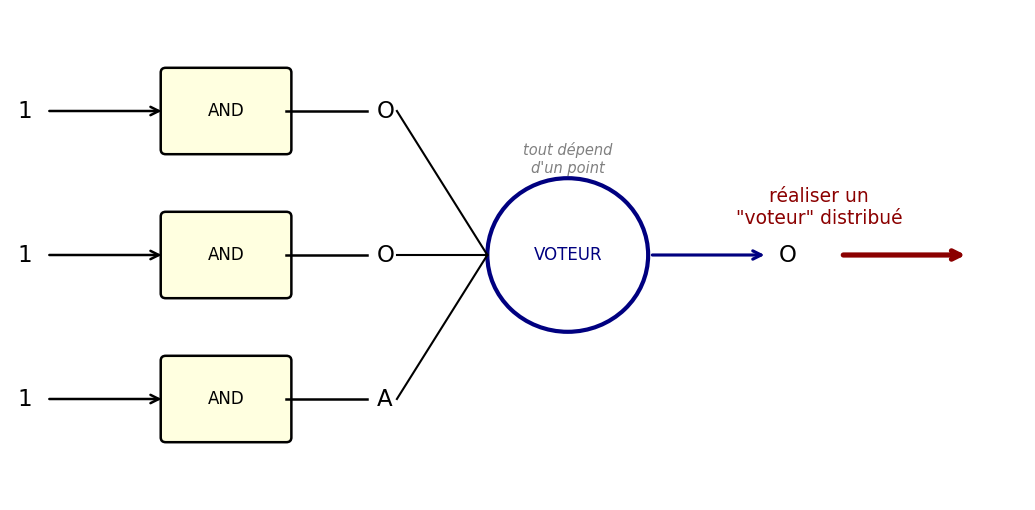
\includegraphics[width=0.72\textwidth]{figures/fig_voter_circuit.png}
  \caption{Schéma d'un voteur centralisé (portes ET/OU) dont l'objectif est d'être
           remplacé par un voteur distribué.}
  \label{fig:voter_circuit}
\end{figure}

\begin{definition}[Problème du consensus byzantin]
Initialement, chaque processus possède une valeur entière. L'objectif est de
concevoir un algorithme réparti à l'issue duquel :
\begin{enumerate}[label=(\roman*)]
  \item Chaque processus non défaillant \emph{décide} une valeur.
  \item Deux processus non défaillants ne décident pas des valeurs différentes.
  \item Si tous les processus non défaillants ont la même valeur initiale, cette
        valeur est la seule valeur de décision possible.
\end{enumerate}
\end{definition}

\subsection{Difficulté du problème}

On démontre successivement :
\begin{enumerate}
  \item Le problème est facile à résoudre dans le cas du \emph{consensus simple}
        (sans byzantins).
  \item Le problème est \emph{difficile} en présence de défaillances byzantines.
  \item Le problème est \emph{impossible} dans un système asynchrone (FLP).
  \item Une solution existe dans le cas \emph{synchrone} avec arrêt total.
\end{enumerate}

Pour illustrer la difficulté, considérons $n = 4$ processus dont un est byzantin.
Le processus byzantin $C$ peut envoyer des valeurs différentes à chacun de ses
voisins, rendant impossible l'accord sans protocole adapté.

\begin{figure}[H]
  \centering
  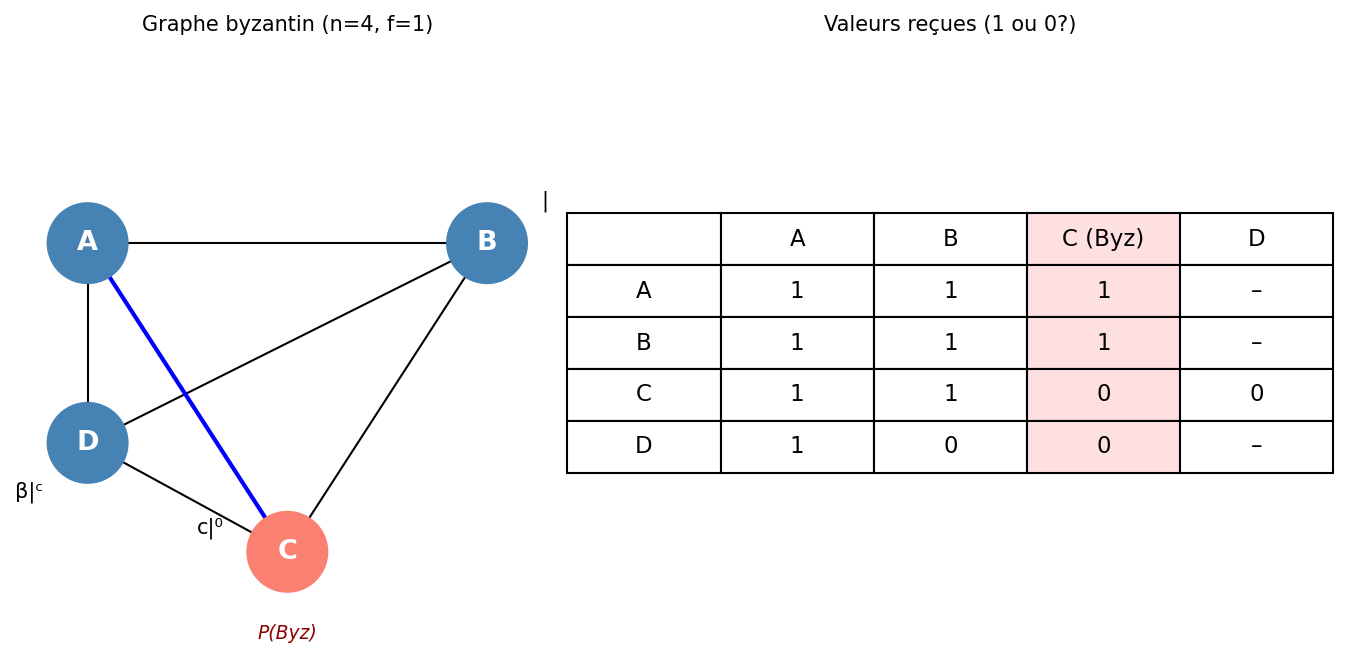
\includegraphics[width=0.82\textwidth]{figures/fig_byzantine_graph.png}
  \caption{Graphe complet à 4 nœuds ($A$, $B$, $C$, $D$) avec $C$ défaillant
           byzantin. La table donne les valeurs reçues par chaque processus ; $C$
           envoie des valeurs incohérentes (0 ou 1 selon le destinataire).}
  \label{fig:byzantine_graph}
\end{figure}

% ─────────────────────────────────────────────────────────────────────────────
\section{Résultat d'impossibilité : Fisher, Lynch, Paterson (FLP)}
% ─────────────────────────────────────────────────────────────────────────────

\begin{theoreme}[FLP, 1985]
Dans un système \emph{asynchrone}, le problème du consensus est impossible, même
avec un seul processus défaillant (arrêt total) et un nombre arbitrairement grand
de processus corrects.
\end{theoreme}

% ─────────────────────────────────────────────────────────────────────────────
\section{Solution synchrone avec défaillances d'arrêt total}
% ─────────────────────────────────────────────────────────────────────────────

\begin{definition}[Flood set]
Soit $f$ une borne supérieure sur le nombre de défaillances, avec $f < n$.
\end{definition}

\noindent\textbf{Algorithme (f+1 phases) :}

Chaque processus exécute $f+1$ phases. Initialement, un processus initialise
un ensemble d'entiers
\[
  \omega := \{\text{valeur initiale}\}.
\]
Chaque processus répète $f+1$ fois :
\begin{itemize}
  \item Envoyer $\omega$ à tous les processus.
  \item Recevoir les $\omega_i$ et faire $\omega := \omega \cup \{\omega_i\}$.
\end{itemize}
À la fin de la phase $f+1$ :
\[
  \text{si } \omega = \{x\} \text{ alors décider } x \;;\quad \text{sinon décider } 0.
\]

\bigskip
\noindent\textbf{Correction de l'algorithme :}

Si tous les processus ont la même valeur initiale, la seule valeur de décision
possible est cette valeur initiale.

Pour le cas général (valeurs initiales distinctes) :

\begin{proposition}
Si à un point de l'exécution les ensembles $\omega_i$ des processus sont égaux,
$(\omega_j = \omega_i,\ j = c)$, alors ils restent égaux jusqu'à la fin du calcul.
Donc tous les processus qui décident, décident la même valeur.
\end{proposition}

\begin{proof}
Il existe au moins une phase au cours de laquelle aucun processus n'est
défaillant (car il y a au plus $f$ défaillances et $f+1$ phases). Lors de cette
phase, chaque processus reçoit le même ensemble de valeurs, donc tous les
$\omega_i$ coïncident à partir de ce point.
\end{proof}

\bigskip
\noindent\textbf{Références :} Lamport, Shosstak, Pease.

\end{document}
